% Options for packages loaded elsewhere
% Options for packages loaded elsewhere
\PassOptionsToPackage{unicode}{hyperref}
\PassOptionsToPackage{hyphens}{url}
\PassOptionsToPackage{dvipsnames,svgnames,x11names}{xcolor}
%
\documentclass[
]{article}
\usepackage{xcolor}
\usepackage[top=0.75in,left=0.75in,bottom=0.75in,right=0.75in]{geometry}
\usepackage{amsmath,amssymb}
\setcounter{secnumdepth}{5}
\usepackage{iftex}
\ifPDFTeX
  \usepackage[T1]{fontenc}
  \usepackage[utf8]{inputenc}
  \usepackage{textcomp} % provide euro and other symbols
\else % if luatex or xetex
  \usepackage{unicode-math} % this also loads fontspec
  \defaultfontfeatures{Scale=MatchLowercase}
  \defaultfontfeatures[\rmfamily]{Ligatures=TeX,Scale=1}
\fi
\usepackage{lmodern}
\ifPDFTeX\else
  % xetex/luatex font selection
\fi
% Use upquote if available, for straight quotes in verbatim environments
\IfFileExists{upquote.sty}{\usepackage{upquote}}{}
\IfFileExists{microtype.sty}{% use microtype if available
  \usepackage[]{microtype}
  \UseMicrotypeSet[protrusion]{basicmath} % disable protrusion for tt fonts
}{}
\makeatletter
\@ifundefined{KOMAClassName}{% if non-KOMA class
  \IfFileExists{parskip.sty}{%
    \usepackage{parskip}
  }{% else
    \setlength{\parindent}{0pt}
    \setlength{\parskip}{6pt plus 2pt minus 1pt}}
}{% if KOMA class
  \KOMAoptions{parskip=half}}
\makeatother
% Make \paragraph and \subparagraph free-standing
\makeatletter
\ifx\paragraph\undefined\else
  \let\oldparagraph\paragraph
  \renewcommand{\paragraph}{
    \@ifstar
      \xxxParagraphStar
      \xxxParagraphNoStar
  }
  \newcommand{\xxxParagraphStar}[1]{\oldparagraph*{#1}\mbox{}}
  \newcommand{\xxxParagraphNoStar}[1]{\oldparagraph{#1}\mbox{}}
\fi
\ifx\subparagraph\undefined\else
  \let\oldsubparagraph\subparagraph
  \renewcommand{\subparagraph}{
    \@ifstar
      \xxxSubParagraphStar
      \xxxSubParagraphNoStar
  }
  \newcommand{\xxxSubParagraphStar}[1]{\oldsubparagraph*{#1}\mbox{}}
  \newcommand{\xxxSubParagraphNoStar}[1]{\oldsubparagraph{#1}\mbox{}}
\fi
\makeatother

\usepackage{color}
\usepackage{fancyvrb}
\newcommand{\VerbBar}{|}
\newcommand{\VERB}{\Verb[commandchars=\\\{\}]}
\DefineVerbatimEnvironment{Highlighting}{Verbatim}{commandchars=\\\{\}}
% Add ',fontsize=\small' for more characters per line
\usepackage{framed}
\definecolor{shadecolor}{RGB}{241,243,245}
\newenvironment{Shaded}{\begin{snugshade}}{\end{snugshade}}
\newcommand{\AlertTok}[1]{\textcolor[rgb]{0.68,0.00,0.00}{#1}}
\newcommand{\AnnotationTok}[1]{\textcolor[rgb]{0.37,0.37,0.37}{#1}}
\newcommand{\AttributeTok}[1]{\textcolor[rgb]{0.40,0.45,0.13}{#1}}
\newcommand{\BaseNTok}[1]{\textcolor[rgb]{0.68,0.00,0.00}{#1}}
\newcommand{\BuiltInTok}[1]{\textcolor[rgb]{0.00,0.23,0.31}{#1}}
\newcommand{\CharTok}[1]{\textcolor[rgb]{0.13,0.47,0.30}{#1}}
\newcommand{\CommentTok}[1]{\textcolor[rgb]{0.37,0.37,0.37}{#1}}
\newcommand{\CommentVarTok}[1]{\textcolor[rgb]{0.37,0.37,0.37}{\textit{#1}}}
\newcommand{\ConstantTok}[1]{\textcolor[rgb]{0.56,0.35,0.01}{#1}}
\newcommand{\ControlFlowTok}[1]{\textcolor[rgb]{0.00,0.23,0.31}{\textbf{#1}}}
\newcommand{\DataTypeTok}[1]{\textcolor[rgb]{0.68,0.00,0.00}{#1}}
\newcommand{\DecValTok}[1]{\textcolor[rgb]{0.68,0.00,0.00}{#1}}
\newcommand{\DocumentationTok}[1]{\textcolor[rgb]{0.37,0.37,0.37}{\textit{#1}}}
\newcommand{\ErrorTok}[1]{\textcolor[rgb]{0.68,0.00,0.00}{#1}}
\newcommand{\ExtensionTok}[1]{\textcolor[rgb]{0.00,0.23,0.31}{#1}}
\newcommand{\FloatTok}[1]{\textcolor[rgb]{0.68,0.00,0.00}{#1}}
\newcommand{\FunctionTok}[1]{\textcolor[rgb]{0.28,0.35,0.67}{#1}}
\newcommand{\ImportTok}[1]{\textcolor[rgb]{0.00,0.46,0.62}{#1}}
\newcommand{\InformationTok}[1]{\textcolor[rgb]{0.37,0.37,0.37}{#1}}
\newcommand{\KeywordTok}[1]{\textcolor[rgb]{0.00,0.23,0.31}{\textbf{#1}}}
\newcommand{\NormalTok}[1]{\textcolor[rgb]{0.00,0.23,0.31}{#1}}
\newcommand{\OperatorTok}[1]{\textcolor[rgb]{0.37,0.37,0.37}{#1}}
\newcommand{\OtherTok}[1]{\textcolor[rgb]{0.00,0.23,0.31}{#1}}
\newcommand{\PreprocessorTok}[1]{\textcolor[rgb]{0.68,0.00,0.00}{#1}}
\newcommand{\RegionMarkerTok}[1]{\textcolor[rgb]{0.00,0.23,0.31}{#1}}
\newcommand{\SpecialCharTok}[1]{\textcolor[rgb]{0.37,0.37,0.37}{#1}}
\newcommand{\SpecialStringTok}[1]{\textcolor[rgb]{0.13,0.47,0.30}{#1}}
\newcommand{\StringTok}[1]{\textcolor[rgb]{0.13,0.47,0.30}{#1}}
\newcommand{\VariableTok}[1]{\textcolor[rgb]{0.07,0.07,0.07}{#1}}
\newcommand{\VerbatimStringTok}[1]{\textcolor[rgb]{0.13,0.47,0.30}{#1}}
\newcommand{\WarningTok}[1]{\textcolor[rgb]{0.37,0.37,0.37}{\textit{#1}}}

\usepackage{longtable,booktabs,array}
\usepackage{calc} % for calculating minipage widths
% Correct order of tables after \paragraph or \subparagraph
\usepackage{etoolbox}
\makeatletter
\patchcmd\longtable{\par}{\if@noskipsec\mbox{}\fi\par}{}{}
\makeatother
% Allow footnotes in longtable head/foot
\IfFileExists{footnotehyper.sty}{\usepackage{footnotehyper}}{\usepackage{footnote}}
\makesavenoteenv{longtable}
\usepackage{graphicx}
\makeatletter
\newsavebox\pandoc@box
\newcommand*\pandocbounded[1]{% scales image to fit in text height/width
  \sbox\pandoc@box{#1}%
  \Gscale@div\@tempa{\textheight}{\dimexpr\ht\pandoc@box+\dp\pandoc@box\relax}%
  \Gscale@div\@tempb{\linewidth}{\wd\pandoc@box}%
  \ifdim\@tempb\p@<\@tempa\p@\let\@tempa\@tempb\fi% select the smaller of both
  \ifdim\@tempa\p@<\p@\scalebox{\@tempa}{\usebox\pandoc@box}%
  \else\usebox{\pandoc@box}%
  \fi%
}
% Set default figure placement to htbp
\def\fps@figure{htbp}
\makeatother





\setlength{\emergencystretch}{3em} % prevent overfull lines

\providecommand{\tightlist}{%
  \setlength{\itemsep}{0pt}\setlength{\parskip}{0pt}}



 


\makeatletter
\@ifpackageloaded{caption}{}{\usepackage{caption}}
\AtBeginDocument{%
\ifdefined\contentsname
  \renewcommand*\contentsname{Table of contents}
\else
  \newcommand\contentsname{Table of contents}
\fi
\ifdefined\listfigurename
  \renewcommand*\listfigurename{List of Figures}
\else
  \newcommand\listfigurename{List of Figures}
\fi
\ifdefined\listtablename
  \renewcommand*\listtablename{List of Tables}
\else
  \newcommand\listtablename{List of Tables}
\fi
\ifdefined\figurename
  \renewcommand*\figurename{Figure}
\else
  \newcommand\figurename{Figure}
\fi
\ifdefined\tablename
  \renewcommand*\tablename{Table}
\else
  \newcommand\tablename{Table}
\fi
}
\@ifpackageloaded{float}{}{\usepackage{float}}
\floatstyle{ruled}
\@ifundefined{c@chapter}{\newfloat{codelisting}{h}{lop}}{\newfloat{codelisting}{h}{lop}[chapter]}
\floatname{codelisting}{Listing}
\newcommand*\listoflistings{\listof{codelisting}{List of Listings}}
\makeatother
\makeatletter
\makeatother
\makeatletter
\@ifpackageloaded{caption}{}{\usepackage{caption}}
\@ifpackageloaded{subcaption}{}{\usepackage{subcaption}}
\makeatother
\usepackage{bookmark}
\IfFileExists{xurl.sty}{\usepackage{xurl}}{} % add URL line breaks if available
\urlstyle{same}
\hypersetup{
  pdftitle={Lab Eleven -- Point Estimation and Resampling},
  colorlinks=true,
  linkcolor={blue},
  filecolor={Maroon},
  citecolor={Blue},
  urlcolor={Blue},
  pdfcreator={LaTeX via pandoc}}


\title{Lab Eleven -- Point Estimation and Resampling}
\author{}
\date{}
\begin{document}
\maketitle


\normalsize

\normalsize

\textbf{Tips}

\begin{itemize}
\tightlist
\item
  Complete the tasks below. Make sure to start your solutions in on a
  new line that starts with ``\textbf{Solution}:''.
\item
  Make sure to use the Quarto Cheatsheet. This will make completing and
  writing up the lab \emph{much} easier.
\item
  Make sure to use ``enter'' to make your code readable, so it doesn't
  run off the page. I switched the Quarto document to automatically
  render to .pdf, so you can see what you're submitting by default. You
  can switch back for the highlighting by moving the html block above
  the pdf block in the YAML header.
\item
  Don't forget that you can copy-and-paste code when you're doing
  something similar as we did in class!
\item
  Make sure to plot all computed probabilities. This is good
  \texttt{ggplot} practice AND will help make sure you don't make a
  mistake when computing the probability.
\end{itemize}

\section{Introduction}\label{introduction}

When performing point estimation, there isn't just one \emph{right}
answer. For example, the Method of Moments (MOM) and Maximum Likelihood
Estimates (MLEs) aren't always the same.

One question that comes up, is why we calculate the sample variance as
\[S_{n-1}^2 = \frac{1}{n-1} \sum_{i=1}^n (X_i -\bar{X})^2,\] when it is
supposed to be the ``average squared distance from the mean, i.e.,
\[S_n^2 = \frac{1}{n} \sum_{i=1}^n (X_i -\bar{X})^2.\]

\section{Comparing Estimators}\label{comparing-estimators}

\subsection{Initial Simulation}\label{initial-simulation}

In this lab, we will explore why we use \(S_{n-1}^2\) and not \(S_n^2\).
To do this, we will generate data from four known distributions:

\begin{itemize}
\tightlist
\item
  Poisson\((\lambda=2)\)
\item
  Binomial\(\left(n=50, p=\frac{5-\sqrt{21}}{10}\right)\)
\item
  Normal\((\mu=0, \sigma=\sqrt{2})\)
\item
  Exponential\(\left(\lambda = \frac{1}{\sqrt{2}}\right).\)
\end{itemize}

\textbf{Remark}: Note that I have selected the parameters so that the
true variance for all four models is 2.

For each distribution, write a loop that completes the following 1000
times. Put \texttt{set.seed(7272)} at the top of your code chunk.

\begin{itemize}
\tightlist
\item
  Generate a sample of size \(n\) from the distribution.
\item
  Calculate and save \(S_{n-1}^2\) and \(S_n^2.\)
\end{itemize}

Start with \(n=20\). Is there evidence that \(S_{n-1}^2\) is a better
estimator than \(S_n^2\)?

Create a plot or combination of plots (using patchwork) to show the
results across all four distributions. Make sure to create a
corresponding table that numerically summarizes the results of the
simulation. You should include \begin{align*}
\textrm{Bias} &= \textrm{Average of Estimates} - \textrm{True Value}\\
\textrm{Precision} &= \frac{1}{\textrm{Variance of Estimates}}\\
\textrm{Mean Square Error} &= \textrm{Bias}^2 + \textrm{Variance of Estimates}.
\end{align*}

\textbf{Solution}

\normalsize

\begin{Shaded}
\begin{Highlighting}[numbers=left,,]
\FunctionTok{set.seed}\NormalTok{(}\DecValTok{7272}\NormalTok{)}

\NormalTok{n.sims }\OtherTok{\textless{}{-}} \DecValTok{1000}
\CommentTok{\# sample size is 20}
\NormalTok{n }\OtherTok{\textless{}{-}} \DecValTok{20}

\CommentTok{\# Poisson}
\NormalTok{S1\_pois }\OtherTok{\textless{}{-}} \FunctionTok{rep}\NormalTok{(}\ConstantTok{NA}\NormalTok{, n.sims)}
\NormalTok{S2\_pois }\OtherTok{\textless{}{-}} \FunctionTok{rep}\NormalTok{(}\ConstantTok{NA}\NormalTok{, n.sims)}

\ControlFlowTok{for}\NormalTok{(i }\ControlFlowTok{in} \DecValTok{1}\SpecialCharTok{:}\NormalTok{n.sims)\{}
\NormalTok{  curr.sample }\OtherTok{\textless{}{-}} \FunctionTok{rpois}\NormalTok{(}\AttributeTok{n=}\NormalTok{n, }\AttributeTok{lambda =} \DecValTok{2}\NormalTok{)}
\NormalTok{  x\_bar }\OtherTok{=} \FunctionTok{mean}\NormalTok{(curr.sample)}
  \CommentTok{\# don\textquotesingle{}t need for (i in 1:n)\{Xi \textless{}{-} curr.sample[i] S1[i] \textless{}{-} (1/(n {-} 1)) * sum((Xi {-} x\_bar)\^{}2) S2[i] \textless{}{-} 1/n * sum((Xi {-} x\_bar)\^{}2)\}, because it\textquotesingle{}s vectorized.}
\NormalTok{  S1\_pois[i] }\OtherTok{\textless{}{-}} \FunctionTok{sum}\NormalTok{((curr.sample }\SpecialCharTok{{-}}\NormalTok{ x\_bar)}\SpecialCharTok{\^{}}\DecValTok{2}\NormalTok{) }\SpecialCharTok{/}\NormalTok{ (n }\SpecialCharTok{{-}} \DecValTok{1}\NormalTok{)}
\NormalTok{  S2\_pois[i] }\OtherTok{\textless{}{-}} \FunctionTok{sum}\NormalTok{((curr.sample }\SpecialCharTok{{-}}\NormalTok{ x\_bar)}\SpecialCharTok{\^{}}\DecValTok{2}\NormalTok{) }\SpecialCharTok{/}\NormalTok{ n}
\NormalTok{  \}}

\CommentTok{\# Binomial}
\NormalTok{p }\OtherTok{\textless{}{-}}\NormalTok{ (}\DecValTok{5}\SpecialCharTok{{-}}\FunctionTok{sqrt}\NormalTok{(}\DecValTok{21}\NormalTok{))}\SpecialCharTok{/}\DecValTok{10}

\NormalTok{S1\_bin }\OtherTok{\textless{}{-}} \FunctionTok{rep}\NormalTok{(}\ConstantTok{NA}\NormalTok{, n.sims)}
\NormalTok{S2\_bin }\OtherTok{\textless{}{-}} \FunctionTok{rep}\NormalTok{(}\ConstantTok{NA}\NormalTok{, n.sims)}

\ControlFlowTok{for}\NormalTok{(i }\ControlFlowTok{in} \DecValTok{1}\SpecialCharTok{:}\NormalTok{n.sims)\{}
\NormalTok{  curr.sample }\OtherTok{\textless{}{-}} \FunctionTok{rbinom}\NormalTok{(}\AttributeTok{n =}\NormalTok{ n, }\AttributeTok{size =} \DecValTok{50}\NormalTok{, }\AttributeTok{prob =}\NormalTok{ p)}
\NormalTok{  x\_bar }\OtherTok{\textless{}{-}} \FunctionTok{mean}\NormalTok{(curr.sample)}
\NormalTok{  S1\_bin[i] }\OtherTok{\textless{}{-}} \FunctionTok{sum}\NormalTok{((curr.sample }\SpecialCharTok{{-}}\NormalTok{ x\_bar)}\SpecialCharTok{\^{}}\DecValTok{2}\NormalTok{) }\SpecialCharTok{/}\NormalTok{ (n }\SpecialCharTok{{-}} \DecValTok{1}\NormalTok{)}
\NormalTok{  S2\_bin[i] }\OtherTok{\textless{}{-}} \FunctionTok{sum}\NormalTok{((curr.sample }\SpecialCharTok{{-}}\NormalTok{ x\_bar)}\SpecialCharTok{\^{}}\DecValTok{2}\NormalTok{) }\SpecialCharTok{/}\NormalTok{ n}
\NormalTok{\}}

\CommentTok{\# Normal}
\NormalTok{S1\_norm }\OtherTok{\textless{}{-}} \FunctionTok{rep}\NormalTok{(}\ConstantTok{NA}\NormalTok{, n.sims)}
\NormalTok{S2\_norm }\OtherTok{\textless{}{-}} \FunctionTok{rep}\NormalTok{(}\ConstantTok{NA}\NormalTok{, n.sims)}

\ControlFlowTok{for}\NormalTok{(i }\ControlFlowTok{in} \DecValTok{1}\SpecialCharTok{:}\NormalTok{n.sims)\{}
\NormalTok{  curr.sample }\OtherTok{\textless{}{-}} \FunctionTok{rnorm}\NormalTok{(}\AttributeTok{n =}\NormalTok{ n, }\AttributeTok{mean =} \DecValTok{0}\NormalTok{, }\AttributeTok{sd =} \FunctionTok{sqrt}\NormalTok{(}\DecValTok{2}\NormalTok{))}
\NormalTok{  x\_bar }\OtherTok{\textless{}{-}} \FunctionTok{mean}\NormalTok{(curr.sample)}
\NormalTok{  S1\_norm[i] }\OtherTok{\textless{}{-}} \FunctionTok{sum}\NormalTok{((curr.sample }\SpecialCharTok{{-}}\NormalTok{ x\_bar)}\SpecialCharTok{\^{}}\DecValTok{2}\NormalTok{) }\SpecialCharTok{/}\NormalTok{ (n }\SpecialCharTok{{-}} \DecValTok{1}\NormalTok{)}
\NormalTok{  S2\_norm[i] }\OtherTok{\textless{}{-}} \FunctionTok{sum}\NormalTok{((curr.sample }\SpecialCharTok{{-}}\NormalTok{ x\_bar)}\SpecialCharTok{\^{}}\DecValTok{2}\NormalTok{) }\SpecialCharTok{/}\NormalTok{ n}
\NormalTok{\}}

\CommentTok{\# Exponential}
\NormalTok{S1\_exp }\OtherTok{\textless{}{-}} \FunctionTok{rep}\NormalTok{(}\ConstantTok{NA}\NormalTok{, n.sims)}
\NormalTok{S2\_exp }\OtherTok{\textless{}{-}} \FunctionTok{rep}\NormalTok{(}\ConstantTok{NA}\NormalTok{, n.sims)}

\ControlFlowTok{for}\NormalTok{(i }\ControlFlowTok{in} \DecValTok{1}\SpecialCharTok{:}\NormalTok{n.sims)\{}
\NormalTok{  curr.sample }\OtherTok{\textless{}{-}} \FunctionTok{rexp}\NormalTok{(}\AttributeTok{n =}\NormalTok{ n, }\AttributeTok{rate =} \DecValTok{1}\SpecialCharTok{/}\FunctionTok{sqrt}\NormalTok{(}\DecValTok{2}\NormalTok{))}
\NormalTok{  x\_bar }\OtherTok{\textless{}{-}} \FunctionTok{mean}\NormalTok{(curr.sample)}
\NormalTok{  S1\_exp[i] }\OtherTok{\textless{}{-}} \FunctionTok{sum}\NormalTok{((curr.sample }\SpecialCharTok{{-}}\NormalTok{ x\_bar)}\SpecialCharTok{\^{}}\DecValTok{2}\NormalTok{) }\SpecialCharTok{/}\NormalTok{ (n }\SpecialCharTok{{-}} \DecValTok{1}\NormalTok{)}
\NormalTok{  S2\_exp[i] }\OtherTok{\textless{}{-}} \FunctionTok{sum}\NormalTok{((curr.sample }\SpecialCharTok{{-}}\NormalTok{ x\_bar)}\SpecialCharTok{\^{}}\DecValTok{2}\NormalTok{) }\SpecialCharTok{/}\NormalTok{ n}
\NormalTok{\}}
\end{Highlighting}
\end{Shaded}

\normalsize

\normalsize

\begin{Shaded}
\begin{Highlighting}[numbers=left,,]
\NormalTok{raw }\OtherTok{\textless{}{-}} \FunctionTok{tibble}\NormalTok{(}
  \AttributeTok{Estimator=} \FunctionTok{rep}\NormalTok{(}\FunctionTok{c}\NormalTok{(}\StringTok{"S1"}\NormalTok{, }\StringTok{"S2"}\NormalTok{), }\AttributeTok{each =} \DecValTok{1000}\NormalTok{, }\AttributeTok{times =} \DecValTok{4}\NormalTok{),}
  \AttributeTok{Distribution=} \FunctionTok{rep}\NormalTok{(}\FunctionTok{c}\NormalTok{(}\StringTok{"Poisson"}\NormalTok{, }\StringTok{"Binomial"}\NormalTok{, }\StringTok{"Normal"}\NormalTok{, }\StringTok{"Exponential"}\NormalTok{), }
                   \AttributeTok{each =} \DecValTok{2000}\NormalTok{),}
  \AttributeTok{Estimate=}\FunctionTok{c}\NormalTok{(S1\_pois, S2\_pois, S1\_bin, S2\_bin, }
\NormalTok{              S1\_norm, S2\_norm, S1\_exp, S2\_exp)}
\NormalTok{)}

\FunctionTok{ggplot}\NormalTok{(raw) }\SpecialCharTok{+}
  \FunctionTok{geom\_boxplot}\NormalTok{(}\FunctionTok{aes}\NormalTok{(}\AttributeTok{x =}\NormalTok{ Estimator,}
                   \AttributeTok{y=}\NormalTok{ Estimate),}
               \AttributeTok{width =} \FloatTok{0.1}\NormalTok{) }\SpecialCharTok{+}
  \FunctionTok{ggtitle}\NormalTok{(}\StringTok{"Distribution of S1 vs S2 across 1000 simulations"}\NormalTok{) }\SpecialCharTok{+}
  \FunctionTok{theme}\NormalTok{(}\AttributeTok{axis.ticks.x =} \FunctionTok{element\_blank}\NormalTok{()) }\SpecialCharTok{+}
  \FunctionTok{facet\_wrap}\NormalTok{(}\SpecialCharTok{\textasciitilde{}}\NormalTok{ Distribution) }
\end{Highlighting}
\end{Shaded}

\pandocbounded{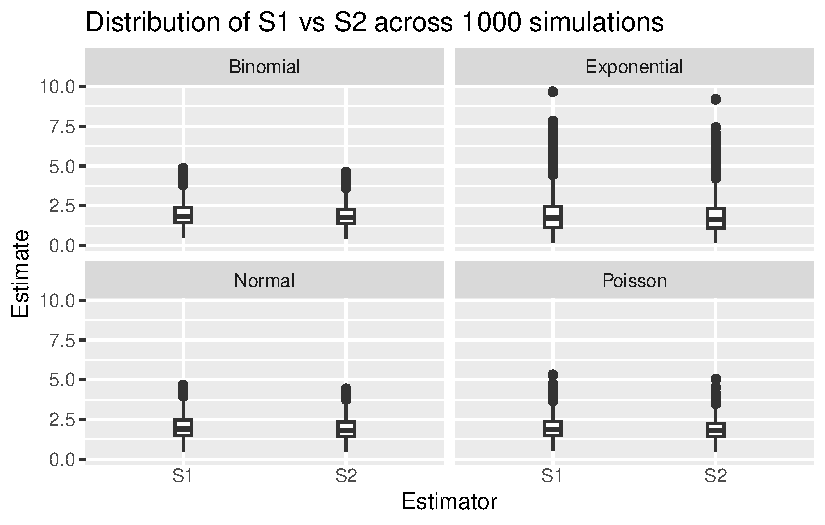
\includegraphics[keepaspectratio]{Lab11WriteUp_files/figure-pdf/unnamed-chunk-3-1.pdf}}

\normalsize

\normalsize

\begin{Shaded}
\begin{Highlighting}[numbers=left,,]
\CommentTok{\# results.S1 \textless{}{-} tibble(}
\CommentTok{\#   Distribution = c("Poisson", "Binomial", "Normal", "Exponential"),}
\CommentTok{\#   Bias = c(}
\CommentTok{\#     mean(S1\_pois) {-} 2,}
\CommentTok{\#     mean(S1\_bin) {-} 2,}
\CommentTok{\#     mean(S1\_norm) {-} 2,}
\CommentTok{\#     mean(S1\_exp) {-} 2}
\CommentTok{\#   ),}
\CommentTok{\#   Variance = c(}
\CommentTok{\#     var(S1\_pois),}
\CommentTok{\#     var(S1\_bin),}
\CommentTok{\#     var(S1\_norm),}
\CommentTok{\#     var(S1\_exp)}
\CommentTok{\#   ),}
\CommentTok{\#   Precision = c(}
\CommentTok{\#     1/var(S1\_pois),}
\CommentTok{\#     1/var(S1\_bin),}
\CommentTok{\#     1/var(S1\_norm),}
\CommentTok{\#     1/var(S1\_exp)}
\CommentTok{\#   ),}
\CommentTok{\#   MSE = c(}
\CommentTok{\#     (mean(S1\_pois) {-} 2)\^{}2 + var(S1\_pois),}
\CommentTok{\#     (mean(S1\_bin) {-} 2)\^{}2 + var(S1\_bin),}
\CommentTok{\#     (mean(S1\_norm) {-} 2)\^{}2 + var(S1\_norm),}
\CommentTok{\#     (mean(S1\_exp) {-} 2)\^{}2 + var(S1\_exp)}
\CommentTok{\#   )}
\CommentTok{\# )}

\NormalTok{results }\OtherTok{\textless{}{-}} \FunctionTok{tibble}\NormalTok{(}
  \AttributeTok{Distribution =} \FunctionTok{rep}\NormalTok{(}\FunctionTok{c}\NormalTok{(}\StringTok{"Poisson"}\NormalTok{, }\StringTok{"Binomial"}\NormalTok{, }\StringTok{"Normal"}\NormalTok{, }\StringTok{"Exponential"}\NormalTok{), }\AttributeTok{each =} \DecValTok{2}\NormalTok{),}
  \AttributeTok{Estimator =} \FunctionTok{rep}\NormalTok{(}\FunctionTok{c}\NormalTok{(}\StringTok{"S1"}\NormalTok{, }\StringTok{"S2"}\NormalTok{), }\AttributeTok{times =} \DecValTok{4}\NormalTok{),}
  \AttributeTok{Bias =} \FunctionTok{c}\NormalTok{(}
    \FunctionTok{mean}\NormalTok{(S1\_pois) }\SpecialCharTok{{-}} \DecValTok{2}\NormalTok{, }\FunctionTok{mean}\NormalTok{(S2\_pois) }\SpecialCharTok{{-}} \DecValTok{2}\NormalTok{,}
    \FunctionTok{mean}\NormalTok{(S1\_bin)  }\SpecialCharTok{{-}} \DecValTok{2}\NormalTok{, }\FunctionTok{mean}\NormalTok{(S2\_bin)  }\SpecialCharTok{{-}} \DecValTok{2}\NormalTok{,}
    \FunctionTok{mean}\NormalTok{(S1\_norm) }\SpecialCharTok{{-}} \DecValTok{2}\NormalTok{, }\FunctionTok{mean}\NormalTok{(S2\_norm) }\SpecialCharTok{{-}} \DecValTok{2}\NormalTok{,}
    \FunctionTok{mean}\NormalTok{(S1\_exp)  }\SpecialCharTok{{-}} \DecValTok{2}\NormalTok{, }\FunctionTok{mean}\NormalTok{(S2\_exp)  }\SpecialCharTok{{-}} \DecValTok{2}
\NormalTok{  ),}
  \AttributeTok{Variance =} \FunctionTok{c}\NormalTok{(}
    \FunctionTok{var}\NormalTok{(S1\_pois), }\FunctionTok{var}\NormalTok{(S2\_pois),}
    \FunctionTok{var}\NormalTok{(S1\_bin),  }\FunctionTok{var}\NormalTok{(S2\_bin),}
    \FunctionTok{var}\NormalTok{(S1\_norm), }\FunctionTok{var}\NormalTok{(S2\_norm),}
    \FunctionTok{var}\NormalTok{(S1\_exp),  }\FunctionTok{var}\NormalTok{(S2\_exp)}
\NormalTok{  ),}
  \AttributeTok{Precision =} \DecValTok{1} \SpecialCharTok{/}\NormalTok{ Variance,}
  \AttributeTok{MSE =}\NormalTok{ Bias}\SpecialCharTok{\^{}}\DecValTok{2} \SpecialCharTok{+}\NormalTok{ Variance}
\NormalTok{)}
\end{Highlighting}
\end{Shaded}

\normalsize

\normalsize

\begin{Shaded}
\begin{Highlighting}[numbers=left,,]
\CommentTok{\# ggplot(results, aes(x = Estimator, y = Bias, fill = Estimator)) +}
\CommentTok{\#   geom\_col() +}
\CommentTok{\#   facet\_wrap(\textasciitilde{} Distribution) +}
\CommentTok{\#   labs(title = "Bias")}

\CommentTok{\# ggplot(results, aes(x = Estimator, y = Precision, fill = Estimator)) +}
\CommentTok{\#   geom\_col() +}
\CommentTok{\#   facet\_wrap(\textasciitilde{} Distribution) +}
\CommentTok{\#   labs(title = "Precision")}

\CommentTok{\# ggplot(results, aes(x = Estimator, y = MSE, fill = Estimator)) +}
\CommentTok{\#   geom\_col() +}
\CommentTok{\#   facet\_wrap(\textasciitilde{} Distribution) +}
\CommentTok{\#   labs(title = "MSE")}
\end{Highlighting}
\end{Shaded}

\normalsize

\normalsize

\begin{longtable}[]{@{}llrrrr@{}}
\toprule\noalign{}
Distribution & Estimator & Bias & Variance & Precision & MSE \\
\midrule\noalign{}
\endhead
\bottomrule\noalign{}
\endlastfoot
Poisson & S1 & -0.02 & 0.48 & 2.10 & 0.48 \\
Poisson & S2 & -0.12 & 0.43 & 2.33 & 0.44 \\
Binomial & S1 & -0.04 & 0.47 & 2.15 & 0.47 \\
Binomial & S2 & -0.13 & 0.42 & 2.38 & 0.44 \\
Normal & S1 & 0.00 & 0.49 & 2.03 & 0.49 \\
Normal & S2 & -0.10 & 0.44 & 2.25 & 0.45 \\
Exponential & S1 & -0.02 & 1.43 & 0.70 & 1.43 \\
Exponential & S2 & -0.12 & 1.29 & 0.77 & 1.30 \\
\end{longtable}

\normalsize

\subsection{Simulation over various sample
sizes}\label{simulation-over-various-sample-sizes}

Consider the effect of the sample size have on these results. Provide a
graphical and numerical summary of what happens as \(n\) increases --
say \(n=20\), \(n=50\), \(n=100\), and \(n=500\). Does the result in
your initial simulation hold across samples? Or, do things change as the
sample size changes? Ensure to set your randomization seed.

\textbf{Solution} Poisson

\normalsize

\begin{Shaded}
\begin{Highlighting}[numbers=left,,]
\FunctionTok{set.seed}\NormalTok{(}\DecValTok{7272}\NormalTok{)}

\NormalTok{n.sims }\OtherTok{\textless{}{-}} \DecValTok{1000}
\NormalTok{ss }\OtherTok{\textless{}{-}} \FunctionTok{c}\NormalTok{(}\DecValTok{20}\NormalTok{, }\DecValTok{50}\NormalTok{, }\DecValTok{100}\NormalTok{, }\DecValTok{500}\NormalTok{)}

\NormalTok{S1\_pois\_n }\OtherTok{\textless{}{-}} \FunctionTok{list}\NormalTok{()}
\NormalTok{S2\_pois\_n }\OtherTok{\textless{}{-}} \FunctionTok{list}\NormalTok{()}

\ControlFlowTok{for}\NormalTok{(n }\ControlFlowTok{in}\NormalTok{ ss)\{}
\NormalTok{  S1 }\OtherTok{\textless{}{-}} \FunctionTok{rep}\NormalTok{(}\ConstantTok{NA}\NormalTok{, n.sims)}
\NormalTok{  S2 }\OtherTok{\textless{}{-}} \FunctionTok{rep}\NormalTok{(}\ConstantTok{NA}\NormalTok{, n.sims)}
  \ControlFlowTok{for}\NormalTok{(i }\ControlFlowTok{in} \DecValTok{1}\SpecialCharTok{:}\NormalTok{n.sims)\{}
\NormalTok{    curr.sample }\OtherTok{\textless{}{-}} \FunctionTok{rpois}\NormalTok{(}\AttributeTok{n =}\NormalTok{ n, }\AttributeTok{lambda =} \DecValTok{2}\NormalTok{)}
\NormalTok{    x\_bar }\OtherTok{\textless{}{-}} \FunctionTok{mean}\NormalTok{(curr.sample)}
\NormalTok{    S1[i] }\OtherTok{\textless{}{-}} \FunctionTok{sum}\NormalTok{((curr.sample }\SpecialCharTok{{-}}\NormalTok{ x\_bar)}\SpecialCharTok{\^{}}\DecValTok{2}\NormalTok{) }\SpecialCharTok{/}\NormalTok{ (n }\SpecialCharTok{{-}} \DecValTok{1}\NormalTok{)}
\NormalTok{    S2[i] }\OtherTok{\textless{}{-}} \FunctionTok{sum}\NormalTok{((curr.sample }\SpecialCharTok{{-}}\NormalTok{ x\_bar)}\SpecialCharTok{\^{}}\DecValTok{2}\NormalTok{) }\SpecialCharTok{/}\NormalTok{ n}
\NormalTok{  \}}
\NormalTok{  S1\_pois\_n[[}\FunctionTok{as.character}\NormalTok{(n)]] }\OtherTok{\textless{}{-}}\NormalTok{ S1}
\NormalTok{  S2\_pois\_n[[}\FunctionTok{as.character}\NormalTok{(n)]] }\OtherTok{\textless{}{-}}\NormalTok{ S2}
\NormalTok{\}}

\CommentTok{\# raw data for boxplots}
\NormalTok{raw\_pois }\OtherTok{\textless{}{-}} \FunctionTok{tibble}\NormalTok{(}
  \AttributeTok{Estimator=} \FunctionTok{rep}\NormalTok{(}\FunctionTok{c}\NormalTok{(}\StringTok{"S1"}\NormalTok{, }\StringTok{"S2"}\NormalTok{), }\AttributeTok{each =} \DecValTok{1000}\NormalTok{, }\AttributeTok{times =} \DecValTok{4}\NormalTok{),}
  \AttributeTok{n=}\FunctionTok{rep}\NormalTok{(ss, }\AttributeTok{each =} \DecValTok{2000}\NormalTok{),}
  \AttributeTok{Estimate=} \FunctionTok{c}\NormalTok{(S1\_pois\_n[[}\StringTok{"20"}\NormalTok{]],  S2\_pois\_n[[}\StringTok{"20"}\NormalTok{]],}
\NormalTok{              S1\_pois\_n[[}\StringTok{"50"}\NormalTok{]],  S2\_pois\_n[[}\StringTok{"50"}\NormalTok{]],}
\NormalTok{              S1\_pois\_n[[}\StringTok{"100"}\NormalTok{]], S2\_pois\_n[[}\StringTok{"100"}\NormalTok{]],}
\NormalTok{              S1\_pois\_n[[}\StringTok{"500"}\NormalTok{]], S2\_pois\_n[[}\StringTok{"500"}\NormalTok{]])}
\NormalTok{)}
\CommentTok{\# summary table}
\NormalTok{results\_pois }\OtherTok{\textless{}{-}} \FunctionTok{tibble}\NormalTok{(}
  \AttributeTok{Samplesize =} \FunctionTok{rep}\NormalTok{(}\FunctionTok{c}\NormalTok{(}\DecValTok{20}\NormalTok{, }\DecValTok{50}\NormalTok{, }\DecValTok{100}\NormalTok{, }\DecValTok{500}\NormalTok{), }\AttributeTok{each=}\DecValTok{2}\NormalTok{),}
  \AttributeTok{Estimator =} \FunctionTok{rep}\NormalTok{(}\FunctionTok{c}\NormalTok{(}\StringTok{"S1"}\NormalTok{, }\StringTok{"S2"}\NormalTok{), }\AttributeTok{times =} \DecValTok{4}\NormalTok{),}
  \AttributeTok{Bias      =} \FunctionTok{c}\NormalTok{(}
    \FunctionTok{mean}\NormalTok{(S1\_pois\_n[[}\StringTok{"20"}\NormalTok{]])  }\SpecialCharTok{{-}} \DecValTok{2}\NormalTok{, }\FunctionTok{mean}\NormalTok{(S2\_pois\_n[[}\StringTok{"20"}\NormalTok{]])  }\SpecialCharTok{{-}} \DecValTok{2}\NormalTok{,}
    \FunctionTok{mean}\NormalTok{(S1\_pois\_n[[}\StringTok{"50"}\NormalTok{]])  }\SpecialCharTok{{-}} \DecValTok{2}\NormalTok{, }\FunctionTok{mean}\NormalTok{(S2\_pois\_n[[}\StringTok{"50"}\NormalTok{]])  }\SpecialCharTok{{-}} \DecValTok{2}\NormalTok{,}
    \FunctionTok{mean}\NormalTok{(S1\_pois\_n[[}\StringTok{"100"}\NormalTok{]]) }\SpecialCharTok{{-}} \DecValTok{2}\NormalTok{, }\FunctionTok{mean}\NormalTok{(S2\_pois\_n[[}\StringTok{"100"}\NormalTok{]]) }\SpecialCharTok{{-}} \DecValTok{2}\NormalTok{,}
    \FunctionTok{mean}\NormalTok{(S1\_pois\_n[[}\StringTok{"500"}\NormalTok{]]) }\SpecialCharTok{{-}} \DecValTok{2}\NormalTok{, }\FunctionTok{mean}\NormalTok{(S2\_pois\_n[[}\StringTok{"500"}\NormalTok{]]) }\SpecialCharTok{{-}} \DecValTok{2}
\NormalTok{  ),}
  \AttributeTok{Variance  =} \FunctionTok{c}\NormalTok{(}
    \FunctionTok{var}\NormalTok{(S1\_pois\_n[[}\StringTok{"20"}\NormalTok{]]),  }\FunctionTok{var}\NormalTok{(S2\_pois\_n[[}\StringTok{"20"}\NormalTok{]]),}
    \FunctionTok{var}\NormalTok{(S1\_pois\_n[[}\StringTok{"50"}\NormalTok{]]),  }\FunctionTok{var}\NormalTok{(S2\_pois\_n[[}\StringTok{"50"}\NormalTok{]]),}
    \FunctionTok{var}\NormalTok{(S1\_pois\_n[[}\StringTok{"100"}\NormalTok{]]), }\FunctionTok{var}\NormalTok{(S2\_pois\_n[[}\StringTok{"100"}\NormalTok{]]),}
    \FunctionTok{var}\NormalTok{(S1\_pois\_n[[}\StringTok{"500"}\NormalTok{]]), }\FunctionTok{var}\NormalTok{(S2\_pois\_n[[}\StringTok{"500"}\NormalTok{]])}
\NormalTok{  ),}
  \AttributeTok{Precision =} \DecValTok{1} \SpecialCharTok{/}\NormalTok{ Variance,}
  \AttributeTok{MSE       =}\NormalTok{ Bias}\SpecialCharTok{\^{}}\DecValTok{2} \SpecialCharTok{+}\NormalTok{ Variance)}

\CommentTok{\# table}
\NormalTok{results\_pois }\SpecialCharTok{|\textgreater{}}\NormalTok{ knitr}\SpecialCharTok{::}\FunctionTok{kable}\NormalTok{(}\AttributeTok{digits =} \DecValTok{2}\NormalTok{)}
\end{Highlighting}
\end{Shaded}

\begin{longtable}[]{@{}rlrrrr@{}}
\toprule\noalign{}
Samplesize & Estimator & Bias & Variance & Precision & MSE \\
\midrule\noalign{}
\endhead
\bottomrule\noalign{}
\endlastfoot
20 & S1 & -0.02 & 0.48 & 2.10 & 0.48 \\
20 & S2 & -0.12 & 0.43 & 2.33 & 0.44 \\
50 & S1 & -0.03 & 0.20 & 5.03 & 0.20 \\
50 & S2 & -0.07 & 0.19 & 5.24 & 0.20 \\
100 & S1 & 0.01 & 0.11 & 9.34 & 0.11 \\
100 & S2 & -0.01 & 0.10 & 9.53 & 0.11 \\
500 & S1 & 0.00 & 0.02 & 52.26 & 0.02 \\
500 & S2 & -0.01 & 0.02 & 52.47 & 0.02 \\
\end{longtable}

\normalsize

\subsection{Simulation}\label{simulation}

You have written code to draw a random sample of various sizes from each
distribution, and to calculate and store the calculated estimates.
Rework your code to produce a density plot of the \(s_{n-1}^2\) and
\(s_{n}^2\). Do you have a guess about their distribution? Ensure to set
your randomization seed.

\subsection{Bootstrap}\label{bootstrap}

Now, take \emph{one} sample from each distribution. Instead of drawing a
random sample at each iteration, sample \emph{with replacement} from the
one sample. Produce a density plot of the \(s_{n-1}^2\) and \(s_{n}^2\).
Do we get roughly the same information as we do in the full simulation?
Try this over several seeds -- what do you notice? Ensure to set your
randomization seed.

\section{Executive Summary}\label{executive-summary}

Summarize the work you've done here to provide a brief (200-300 word)
summary of the simulation and the results using your work in Lab 11.
Your summary should be professional, clear, and all claims should be
corroborated with statistical support.




\end{document}
